\renewcommand{\thepage}{}
\chapter{The project plan}
\thispagestyle{empty}
\pagestyle{fancy}
\lhead{\small \bf  Chapter 4: The project plan}
\rhead{}
\chead{}
\renewcommand\thepage{\arabic{page}}
 \setcounter{minitocdepth}{1}
\minitoc
\clearpage
\section{Introduction}
\lettrine[lines=2,lhang=0.44,lraise=0,loversize=0.08,findent=-0.11em,slope=0.6em]%
{T}{} he work that has lead us to achieve the application has been managed as a project. To be successful a project must:
\begin{itemize}[font=\color{black}, label=\maltese]
\item Deliver the outcomes and benefits required by the organization, its delivery partners and other stakeholder organizations;
\item Create and implement deliverables that meet agreed requirements;
\item Meet time targets;
\item Stay within financial budgets;
\item Involve all the right people;
\item Make best use of resources in the organization and elsewhere;
\item Take account of changes in the way the organization operates;
\item Manage any risks that could jeopardize success;
\item Take into account the needs of staff and other stakeholders who will be impacted by the changes brought about by the project.
\end{itemize}
\paragraph*{}
In order to manage effectively it helps to understand the typical lifecycle of a project and how it applies to our specific one. One needs to decide how the management activities of the lifecycle steps will be achieved, and precisely who will be involved. One must make sure he understands his role in making these things happen in the right way and at the right time.\\
Much of the project management effort across the lifecycle are driven by the owner/sponsor of the project (known as the Senior Responsible Owner (SRO) ), and the Project Manager. To achieve success they will almost certainly need to draw upon the skills and experience of many others from within the organization, its partners and suppliers.
\begin{figure}[h]
\centering
\includegraphics[scale=0.6, frame]{p-lifecycle.jpg}
\caption{The project life cycle}
\end{figure}
\paragraph*{}
While Step 3 - Running a Project is by far the most resource intensive part of the project, it is the care and effort devoted to project start up and initiation that makes the most significant contribution to project success. The success of a project critically depends upon the effort, care and skill one applies in its initial planning.
\paragraph*{}
In this chapter we present the methodology adopted for the development, thereafter we explain our progress work and we wind up with the backlog Product.
\section{Methodology and software development life cycle}
\paragraph*{}
Managing a project requires a precise methodology that depends on its size and type. For small projects that the domain is well known, a Waterfall life cycle [W8] is very suitable.
All of the business requirements are well known from the beginning of the project and the Waterfall life cycle is able to handle requirements that are intended to extend the project. When the domain of interest of the project is mastered and if its size is important one must rather use a V-model life cycle[W9]. If all of the requirements are not well known or some of them are unclear, an iterative life cycle [W10] is mandatory.
\paragraph*{}
Stradfi SA has clearly expressed that all of the requirements are not clearly defined and some of them may change. Thus we agreed on the usage of an iterative life cycle. Since the team involved in the development of the $IG�$ application is small and there one have decided a daily communication about the progress of the project and the issues encountered, the SCRUM [W11] methodology becomes the best choice. 
\subsection{SCRUM's presentation}
\paragraph*{}
Agile software development processes are influenced by best practices in Japanese industry, particularly by lean development principles [10] implemented at companies like Toyota [11] and Honda [12], and knowledge management strategies developed by Takeuchi and Nonaka [13], now at the Hitotsubashi Business School in Japan, and Peter Senge [14] at MIT. Scrum is an Agile methodology that delivers software to customer and end users faster, better, and cooler [15] [16].
\paragraph*{}
Scrum works because it optimizes the development environment, reduces organizational overhead, and closely synchronizes market requirements with early feature delivery. Based in modern process control  theory, Scrum produces the best possible software given the available resources, acceptable quality levels, and required release dates. At its core, Scrum is an iterative, incremental process for developing any product or managing any work that produces a potentially shippable set of functionality at the end of each iteration. Scrum's attributes are:
\begin{itemize}
\item Scrum is an agile process to manage and control development work.
\item Scrum is a wrapper for existing engineering practices.
\item Scrum is a team-based approach to developing systems when requirements are changing rapidly.
\item Scrum controls the chaos of conflicting interests and needs.
\item Scrum improves communication and maximizes cooperation.
\item Scrum detects and removes anything that gets in the way of developing and delivering products.
\item Scrum is a way to maximize productivity.
\item Scrum scales from single projects to entire organizations, and has managed development for multiple interrelated products and projects with over a thousand team members.
\item Scrum is a way for everyone to feel good about their job, their contributions, and know they have done the very best they possibly could.
\end{itemize}
\paragraph*{}
The method is characterized by the production of a Product Backlog where requested features are organized by their priority (Figure IV.2). A Product Owner is responsible for approving changes to the product backlog. Implementation occurs in roughly 30 day iterations called Sprints which focus on the top priorities in the Product Backlog. The goal of each Sprint is to deliver a potentially shippable product increment. During the Sprint, checkpoints are observed in a daily "Scrum" meeting which communicates the progress and activities within the team and shares issues that may be "blocking" progress for an individual or the team. This allows the Scrum Master to determine progress against the Sprint commitments and advise on midcourse corrections to assure successful completion of the Sprint.
\newpage
\begin{figure}[h]
\begin{center}
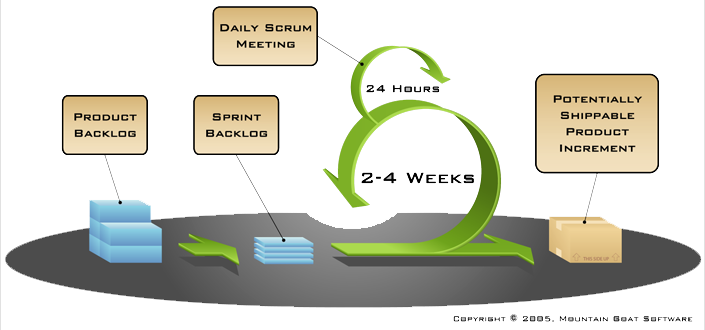
\includegraphics[scale=0.5, frame]{cycle-scrum.png}
\end{center}
\caption{The Scrum process}
\end{figure}
\subsubsection{Scrum Principles}
\paragraph*{}
While those are some of the mechanics of Scrum, more importantly, one should understand that Scrum is guided by a few key principles: 
\begin{itemize}
\item The belief that effective software development is best implemented via an empirical rather than planned process; 
\item The belief that, once organizational impediments are removed, a self organizing and self managing team will naturally deliver better software than would otherwise be the case; 
\item The premise that you can deliver the most valuable software within a prescribed time and budget, and yet you cannot definitively predict the exact functionality of what a team will deliver.
\end{itemize}
\paragraph*{}
Scrum's assertion is that recognizing these key principles frees an organization from many of the constraints that prevent effective software development. However, one must also recognize that these key principles imply potentially significant change to the organization that chooses to adopt them. Since these principles form the underlying basis of Scrum, each merits some additional discussion.
\subsubsection{Adopting an Empirical vs. Planned Process}
\paragraph*{}
Scrum believes that most systems development today has an incorrect philosophical basis, that is, through more and better planning we can achieve more predictable, higher quality results. Scrum recognizes that the applications development process is an unpredictable and extraordinary complicated process (think hundreds of thousands of manually created lines of code) whose value can only be measured empirically. After all, the application under development has likely not been developed by any team anywhere, ever, much less by your team in your context, so cookbook, step-by-step planning approaches cannot effectively address the inherent unpredictability. Scrum defines the systems development process as a loose set of activities that combines known, workable tools and techniques with an empowered team that is tightly coupled to the Customer/Product Owner. Since many of these activities are loose, controls are applieded such as constant inspection and demonstration  to manage the risk and provide real time, empirical evidence of the state of the project at every point in time.
\paragraph*{}
\textbf{The Scrum tradeoff is simple:} \textit{Know where you are every day with Scrum - or - Think you know where you are on your well-formed plan and discover that you are very wrong, very much later}
\subsubsection{Scrum and Software Agility}
\paragraph*{}
Scrum has been in use since the mid 1990s and has now been applied to thousands of projects worldwide. In addition to Scrum, several new iterative methodologies have also received attention during this period. Like Scrum, each had a combination of old ideas and new ideas, but they all emphasized:
\begin{itemize}
\item Close collaboration between the development team and business experts;
\item Face-to-face communication (as more efficient than written documentation);
\item Frequent delivery of new deployable business value software;
\item Tight, self-organizing teams; and
\item Ways to craft the code and the team to allow for continuous adaptation to changing requirements. 
\end{itemize}
\paragraph*{}
In 2001, various originators and practitioners of these methodologies, including Scrum leaders, met to understand what it was they had in common. They picked the word "agile" for an umbrella term and crafted the "Manifesto for Agile Software Development", its most important aspect being a statement of shared values: \textit{We are uncovering better ways of developing software by doing it and helping others do it. Through this work we have come to value:}
\begin{itemize}
\item Individuals and interactions over processes and tools
\item Working software over comprehensive documentation
\item Customer collaboration over contract negotiation
\item Responding to change over following a plan
\end{itemize}
\paragraph*{}
The Manifesto struck a chord and it led to the start of thousands of new agile projects. The results and experiences of these projects further enhanced the techniques applied by the multiple forms of agile practices. As with any human endeavor, some succeeded and some failed. But what was most striking about the successes was how much both the business people and the technical people loved their project. This was the way they wanted software development done and the customers and end users agreed. Successful projects spawned more enthusiasts and like a successful Sprint, the virtuous agile cycle continues today.
\section{The $IG�$ project management}
\paragraph*{}
The project has been initiated by a kick-off meeting (done by a phone call). The initial project plan has been defined and is presented in the GANTT chart (fig. VI.3). Despite the methodology we tried to stuck as much as we can to this project plan.
\begin{center}
\begin{landscape}
\vspace*{\fill}
\begin{figure}[hbtp]
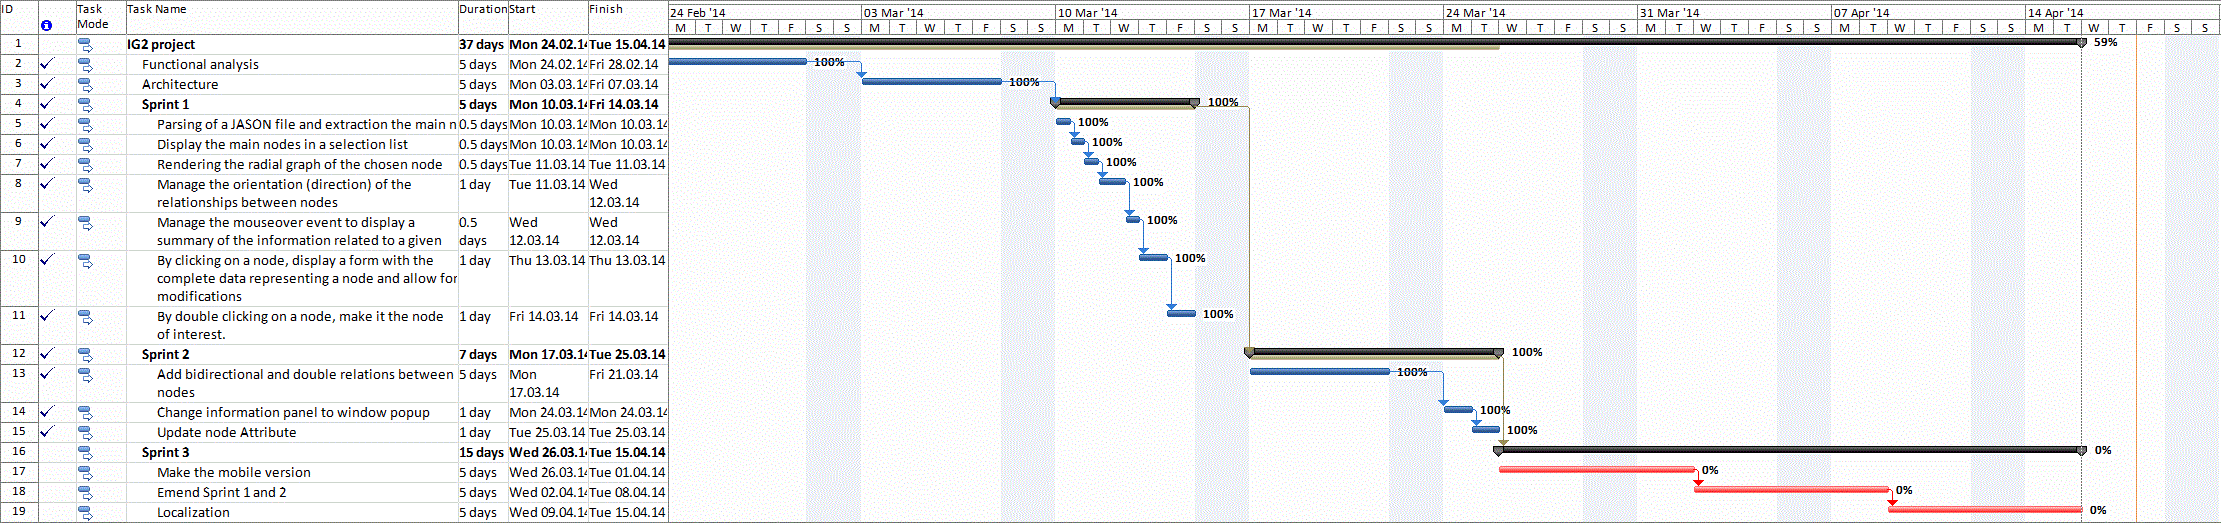
\includegraphics[scale=0.3, frame]{IG2_Manel_A.png}
\caption{The $IG�$ project plan}
\end{figure}
\vspace*{\fill}
\end{landscape}
\end{center}
\newpage
\begin{figure}[h]
\centering
\includegraphics[width=\hsize , frame]{IG2_P1.png}
\caption{List of scheduled tasks}
\end{figure}

%\newpage
%\begin{figure}[!h]
%\centering
%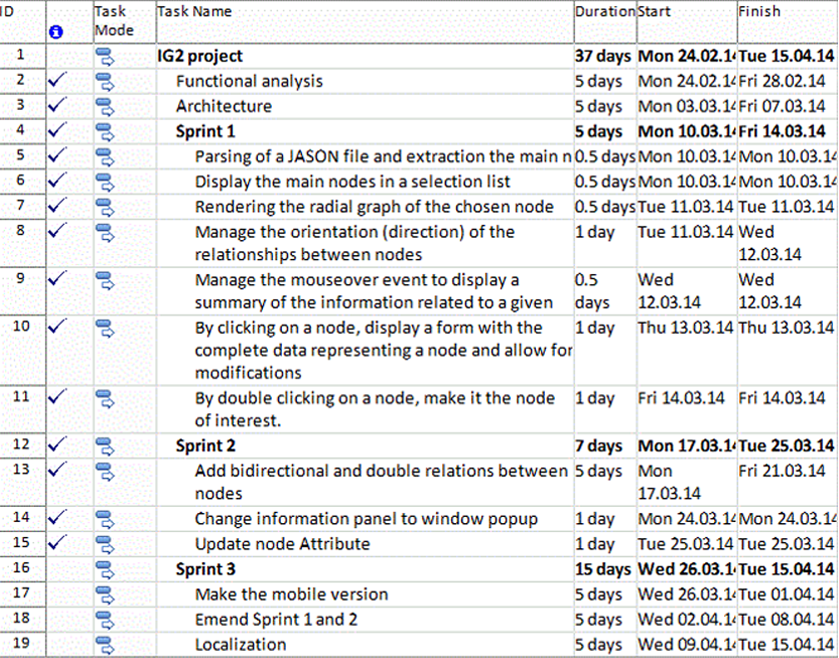
\includegraphics[scale=0.3]{IG2_P11.png}
%\caption{Schedule Sprint}
%\end{figure}
%
%\begin{figure}[!h]
%\centering
%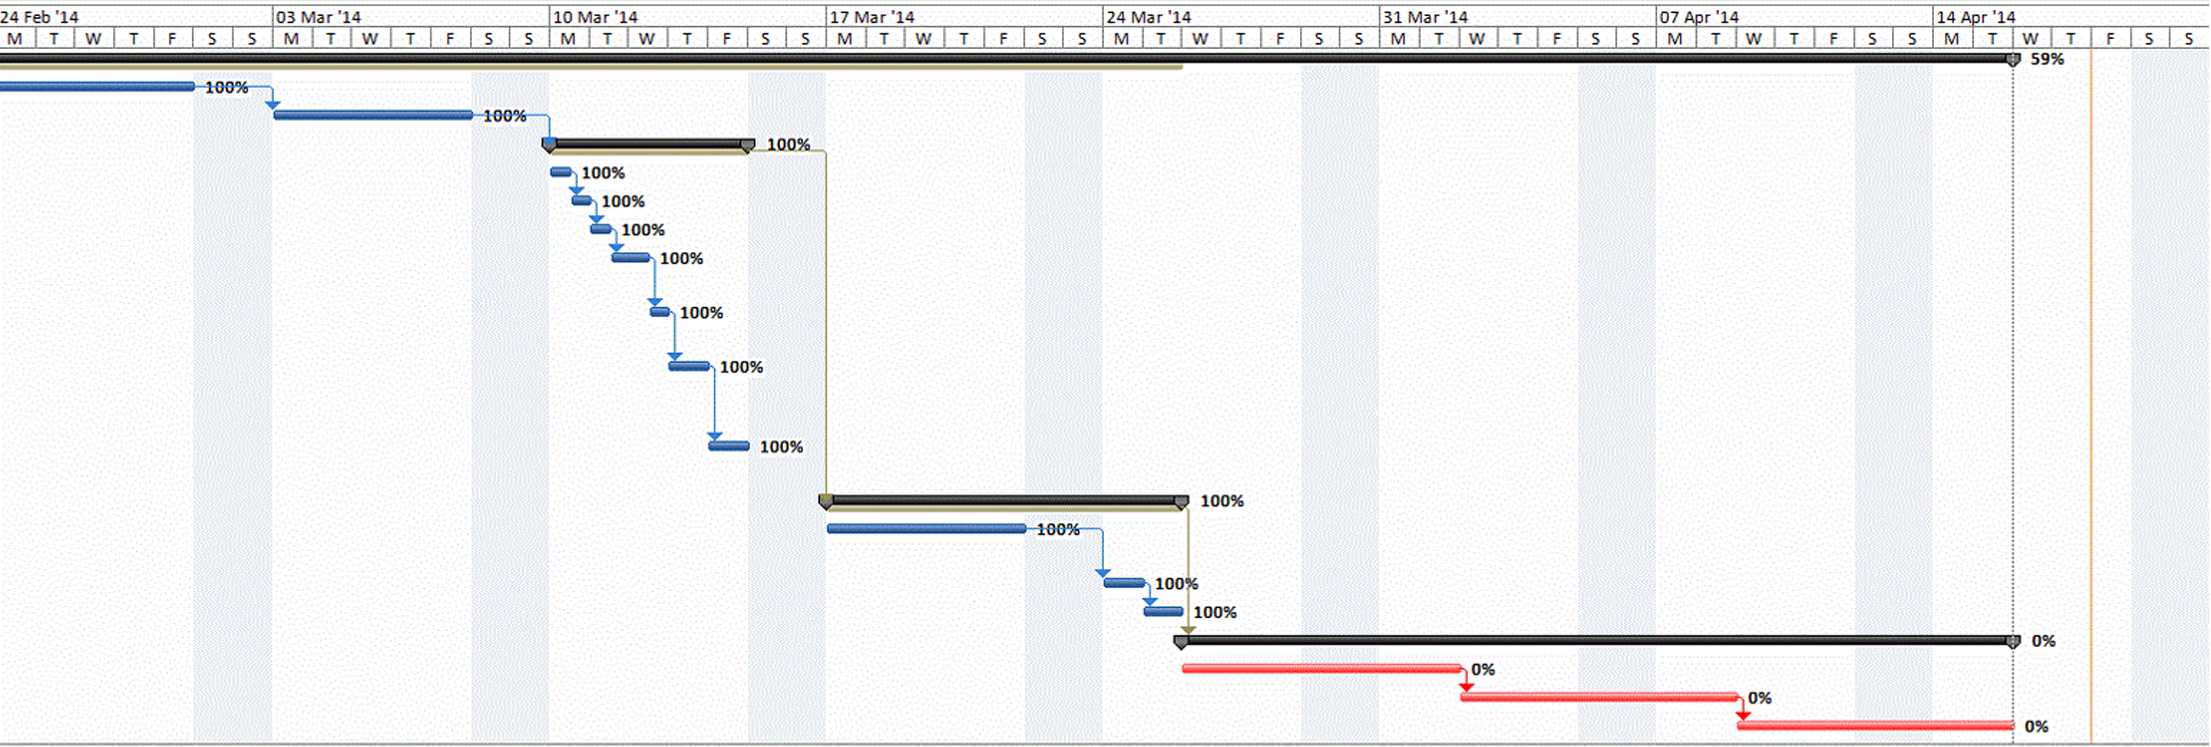
\includegraphics[scale=0.2]{IG2_P22.png}
%\caption{GANTT diagram}
%\end{figure}
\paragraph*{}
The project in its current state was achieved in three sprints. In the first sprint the development environment has been prepared, and a prototype allowing to parse a JSON file and to visualize a radial graph was developed. More details can be found the (paragraph of the 1st sprint). In the second sprint we mainly focused on the management of the nodes and the relations. The update node/relation was a significant part of this sprint.
While developing the second sprint of the project I suggested to the team to localize the user interface. The $IG�$ application is dedicated to an international market and it is very important to allow different people to use it in their mother tongue. Stradfi SA team has appreciated the idea and has expressed its interest to realize this feature in the 3rd sprint.
\section{The overall list requirements}
\paragraph*{}
The product backlog represents the list of the requirements to implement. At the beginning of the project, not all of the requirements are known. Thus some modifications may occur by adding and/or removing some requirements. However, the product owner is asked to prioritize the mastered requirements in order to prepare each sprint's backlog. The following table presents the detailed product backlog in its final form as discussed with team.
\begin{table}[h]
\begin{tabular}{|p{15cm}|}
\hline
\textbf{List} \\
\hline
1.Kick-off meeting \\
\hline
2. Server configuration  \\
\hline
3. Creating oh th JSON files  \\
\hline
4. Architecture and methodology approval \\
\hline
5. Parsing of JSON file \\
\hline
6. Listing of the available objects \\
\hline
7. Rendering the Radial Graph of the selected object \\
\hline
8. Managing the orientation (direction) of the relationships between nodes \\
\hline
9. Implementation of the mouseover event to display a summary of the information related to a given node \\
\hline
10. Accessing to a node attributes and properties \\
\hline
11. Selection of the node of interest \\
\hline
12. Implementation of different types of relations \\
\hline
13. Implementing the features allowing to update the properties and attributes of a given node \\
\hline
14. Implementation the support of different languages \\
\hline
15. Implementing the zoom in and zoom out feature \\
\hline
16. Implementing Drag and Drop capablity \\
\hline
17. Implementing the responsivity \\
\hline
17. Implementing the mouseover support for edges \\
\hline
19. Manage Dropdown list for Type, Aspect and Salutation attribute \\
\hline
\end{tabular}
\caption{The list of Requirements}
\end{table}
\paragraph*{}
The list of requirements shown above has been organized, prioritized and implemented in four sprints. The details of each of them is presented in the next chapter. 
\section{Conclusion}
\paragraph*{}
The kick-off meeting was really very helpful for the project initiation. It clarified things that are very important to achieve a project such as the methodology to adopt and product backlog. This gives the departure signal for the development that has been also done according to the different sprints described above. The overall project plan was also defined during the kick-off meeting and approved during the sprint "zero". The detailed aspects of the implementation are discussed in the next chapter.